%!TEX ROOT=ctutest.tex
\chapter{Testování systému}
    V rámci práce byly také provedeny dva experimenty na simulátoru vibrací (obrázek \ref{figure:motor}), jež slouží pro účely předmětu Diagnostika a testování.\\
    První rotační soustava, na které byly experimenty prováděny, je tvořena stejnosměrným motorem, ložiskem bez poruchy (ložisko 2), hřídelí a poškozeným ložiskem s trhlinou na vnějším kroužku (ložisko 1). Druhá soustava s oběma ložiskami bez poruchy bohužel nebyla funkční, a nemohla tak posloužit jako reference stavu bez poškození, a proto jsme nedokázali určit, jak moc jsou vibrace způsobené trhlinou z prvního ložiska přenášeny přes hřídel na druhé ložisko.\\
    Akcelerometr byl v obou případech připevněn na ložisko tak, aby měřil vibrace v ose kolmé k ose motoru.

     \begin{figure}[!ht]
            \centering
    	    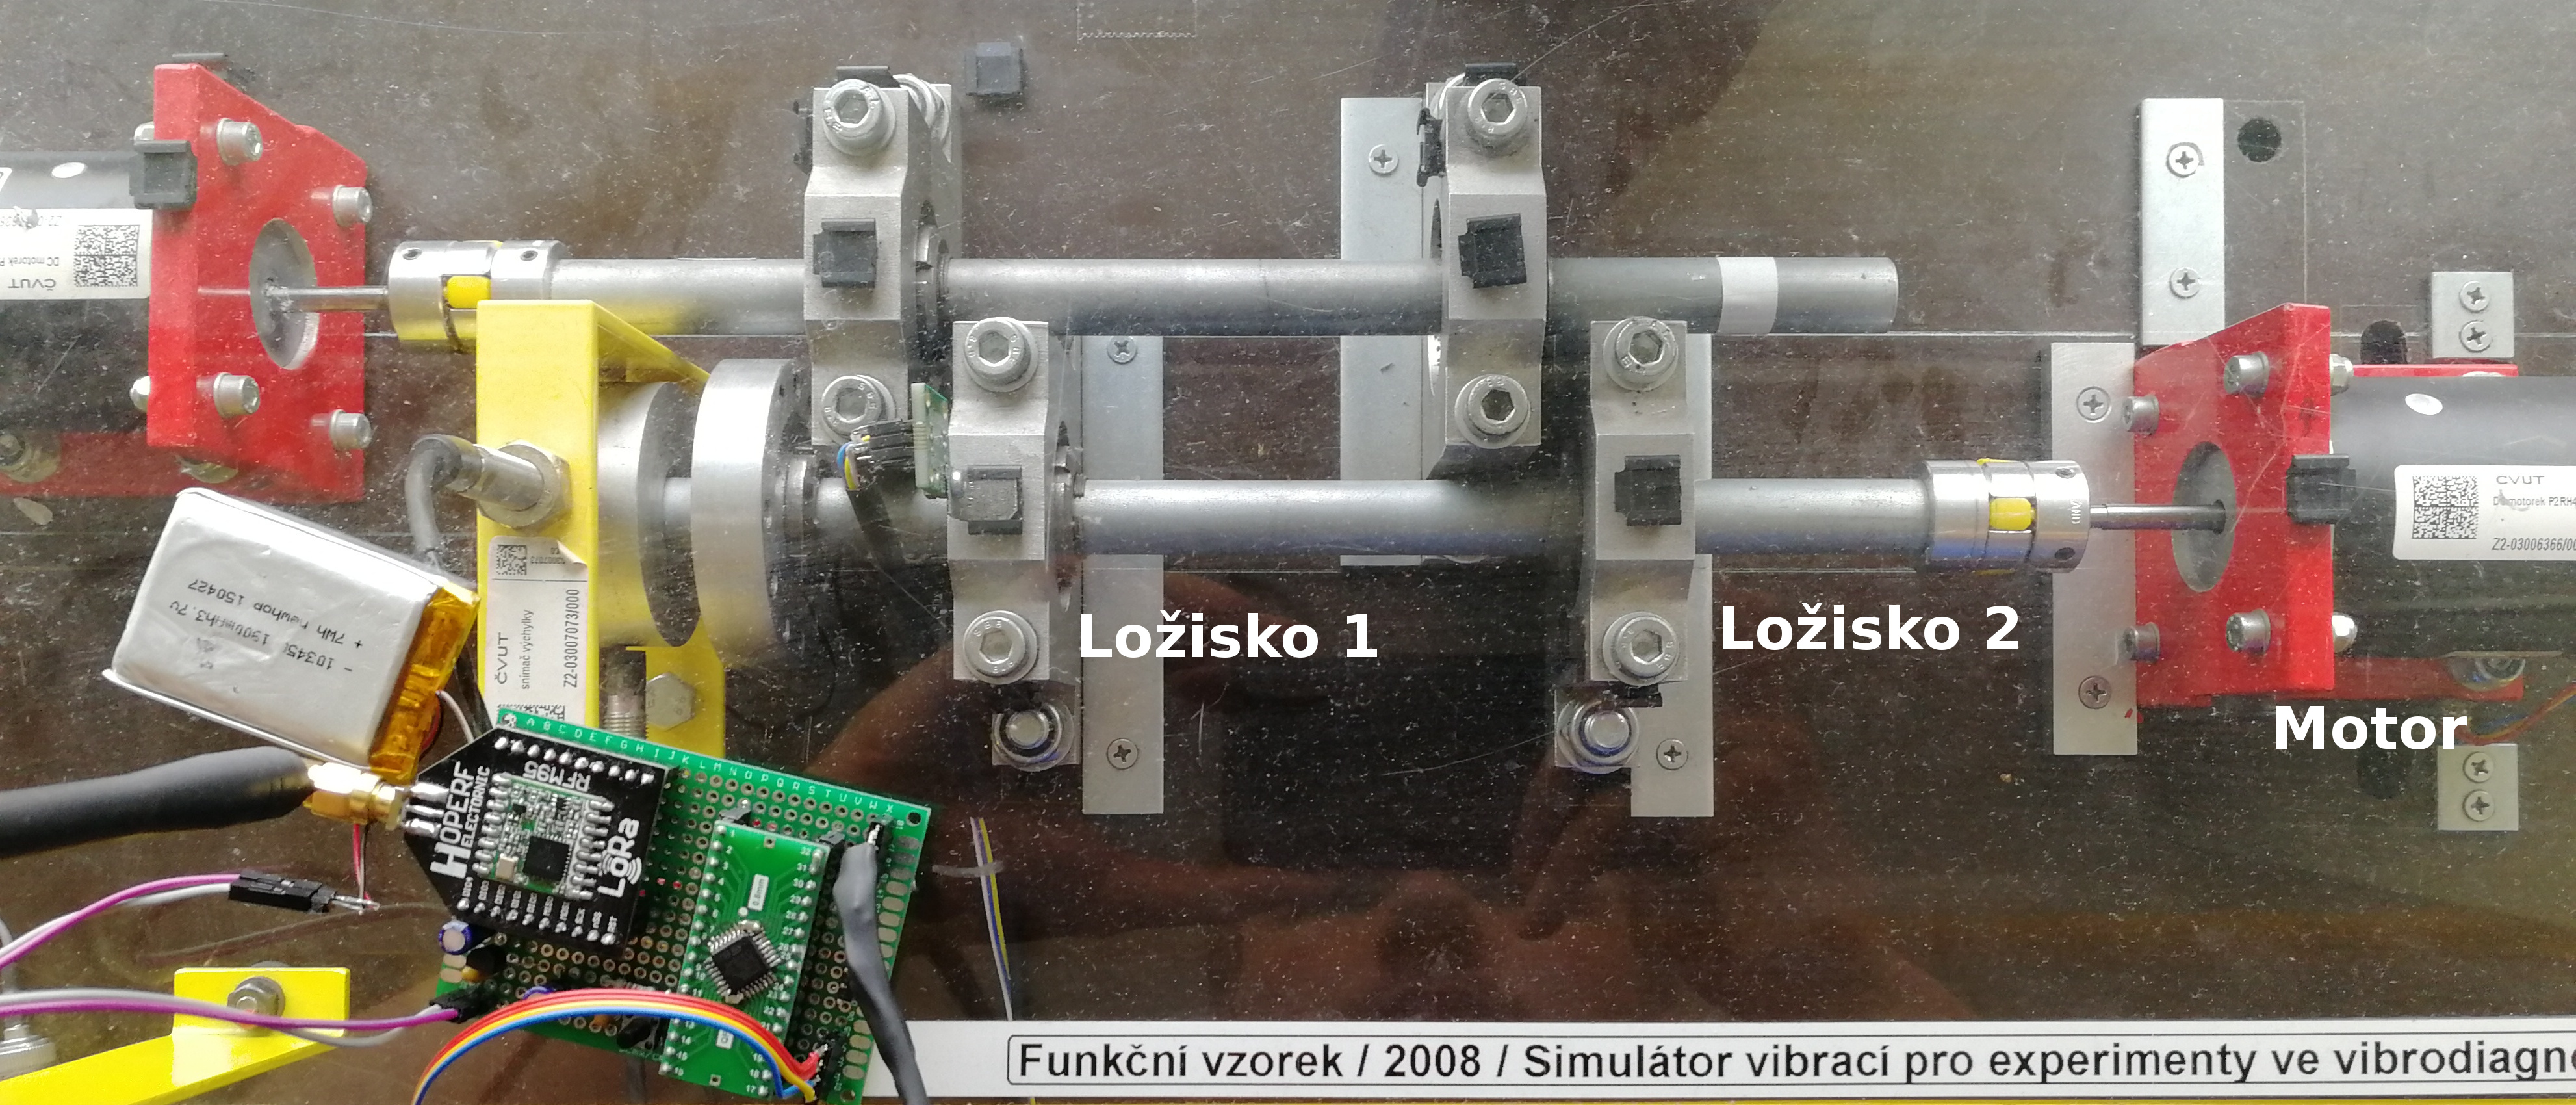
\includegraphics[width =\textwidth]{Experiment/Figs/soustava_best.jpg}
            \caption {Rotační zařízení včetně navržené měřicí jednotky.}
            \label{figure:motor}
    \end{figure}  
    \section{První experiment – nevyváženost osy}
        V prvním experimentu jsme se snažili pomocí analyzovaných příznaků detekovat nevyváženost osy, kdy byl vsazen do válcového tělesa upevněného k hřídeli nevyvážek (šroub), a způsobil tak její drobné vychylování.
        Motor byl roztočen na 3000 otáček za minutu, vzorkovací frekvence AD převodníku byla nastavena na 1.5 kHz, FFT se vypočítávalo z 1024 vzorků, data byla odesílána do centrální jednotky v desetisekundových intervalech.\\
        Nejdříve bylo druhé ložisko monitorováno bez šroubu. Následně byl systém pozastaven (lze vidět na grafech v obrázku \ref{figure:experiment_graphs01}), do kola byl vsazen šroub a v~monitorování se pokračovalo. Na závěr bylo pro případ se šroubem i bez něj v debugovacím módu aplikace odesláno celé amplitudové spektrum.
        
        \begin{figure}[!ht]
            \centering
    	    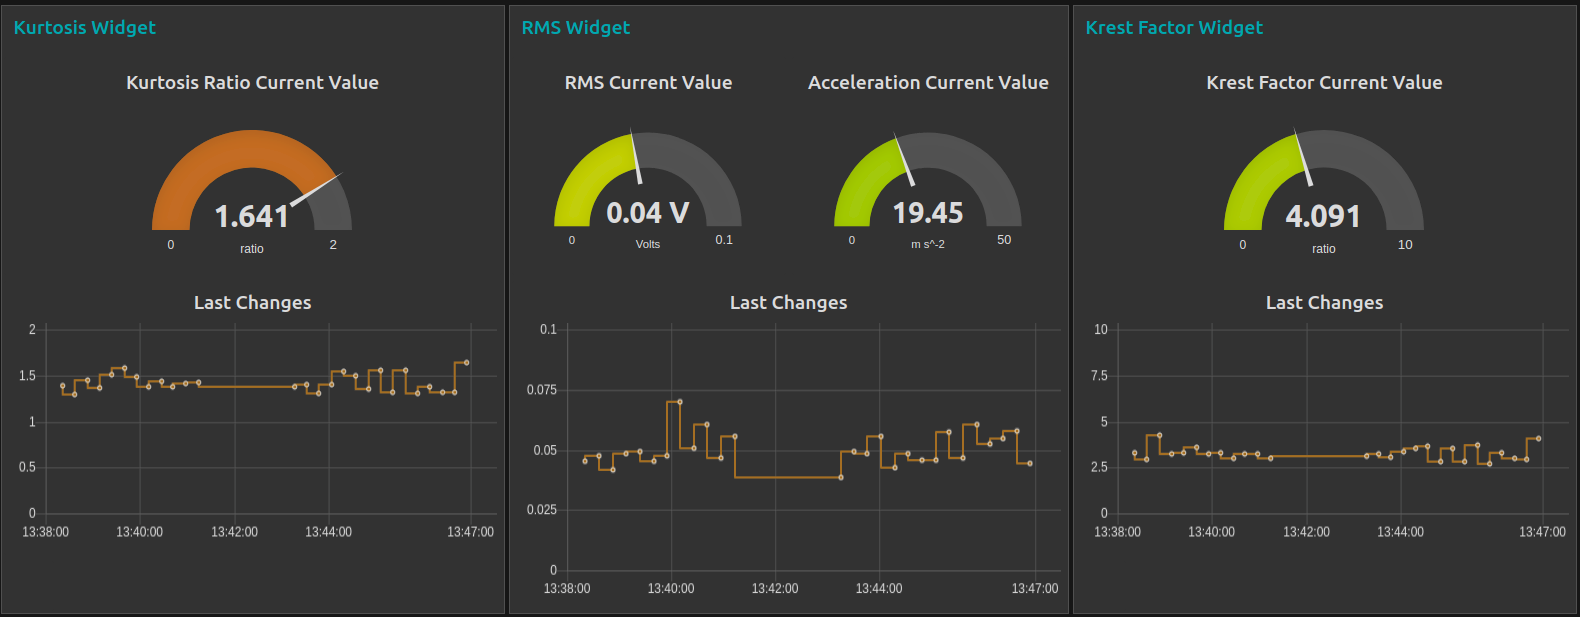
\includegraphics[width=\textwidth]{Experiment/Figs/timechanges_motor_nail.png}
            \caption {První experiment – časový průběh RMS, krest faktoru a kurtosis ratio.}
            \label{figure:experiment_graphs01}
        \end{figure}
        
        \begin{figure} [!htp]
            \centering
            \caption{První experiment – amplitudová spektra.}
            \begin{subfigure}[b]{0.48\textwidth}
                 \centering
                 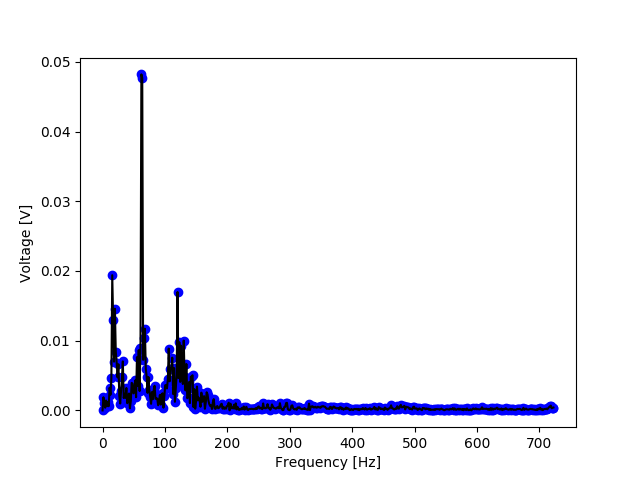
\includegraphics[width=\textwidth]{Experiment/Figs/3000_rpm_1khz_ok.png}
                 \caption {Amplitudové spektrum před vsazením šroubu.}
                 \label{figure:amplitude_01}
             \end{subfigure}
             \hfill
            \begin{subfigure}[b]{0.48\textwidth}
                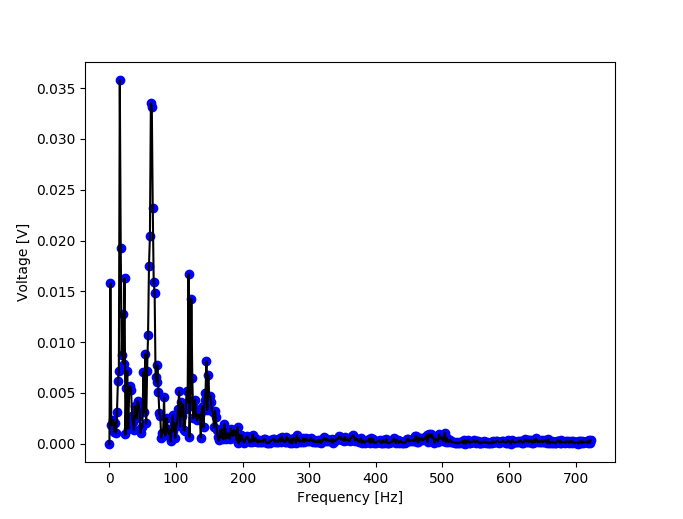
\includegraphics[width=\textwidth]{Experiment/Figs/3000_rpm_1khz_nail.png}
                \caption {Amplitudové spektrum po vsazení šroubu.}
                \label{figure:amplitude_02}
            \end{subfigure}
        \end{figure} 
    
    \subsection{Výsledky}
        Z hlediska příznaků pracujících s vibračním signálem v časové oblasti experiment ukázal, že pro přítomnost šroubu, a tím vzniklou nevyváženost osy, nejsou monitorované veličiny, krest faktor a kurtosis ratio příliš směrodatné. Hodnoty krest faktoru a kurtosis ratio spíše poskytuje informace o poruchách, které způsobují občasné impulsy s nadměrnou amplitudou (kapitoly \ref{section:kurtosis} a \ref{section:krest}).\\ 
        V amplitudovém spektru vibrací před vložením šroubu (obrázek \ref{figure:amplitude_01}) byl nejvýznamnější pík na 53 Hz, který zhruba odpovídal otáčkám motoru 3000 RPM, a 110 Hz odpovídající první harmonické frekvenci. Třetí nejvýraznější pík se nacházel na frekvenci 16 Hz a jeho původ se nepodařilo objasnit. Mohl souviset s přítomností trhliny na poškozeném ložisku nebo s vlastními rezonancemi soustavy.
        Vsazení šroubu se na amplitudovém spektru jasně projevilo, přibylo mnoho nových extrémů, které byly dokonce výraznější než původních 53 Hz (obrázek \ref{figure:amplitude_02}).\\
        Frekvenční spektrum tak opravdu podává mnohem komplexnější informace nežli časové průběhy, což potvrdilo závěry v kapitole \ref{section:techniky}.
    
            
    \section{Druhý experiment – přítomnost trhliny ve vnějším kroužku ložiska}
        V druhém experimentu jsme se snažili pomocí analyzovaných příznaků detekovat přítomnost trhliny na prvním ložisku. Trhlina způsobuje výskyt drobných impulsů v signálu, které by měly ovlivňovat hodnoty průběhů krest faktoru a kurtosis ratio.\\
        Parametry motoru a měřicí jednotky byly nastaveny stejně jako v prvním experimentu.\\
        Nejdříve bylo monitorováno první ložisko s trhlinou, poté byl systém pozastaven a akcelerometr umístěn na druhé ložisko a v~monitorování se pokračovalo. Na závěr bylo opět v obou dvou případech odesláno celé amplitudové spektrum.
        
        \begin{figure} [!hbp]
            \centering
            \caption{Druhý experiment – amplitudová spektra.}
            \begin{subfigure}[b]{0.48\textwidth}
                 \centering
                 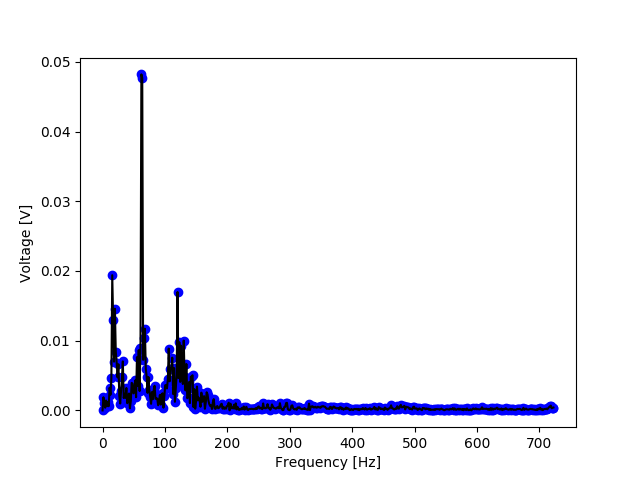
\includegraphics[width=\textwidth]{Experiment/Figs/3000_rpm_1khz_ok.png}
                 \caption {Amplitudové spektrum nepoškozeného ložiska.}
             \end{subfigure}
             \hfill
            \begin{subfigure}[b]{0.48\textwidth}
                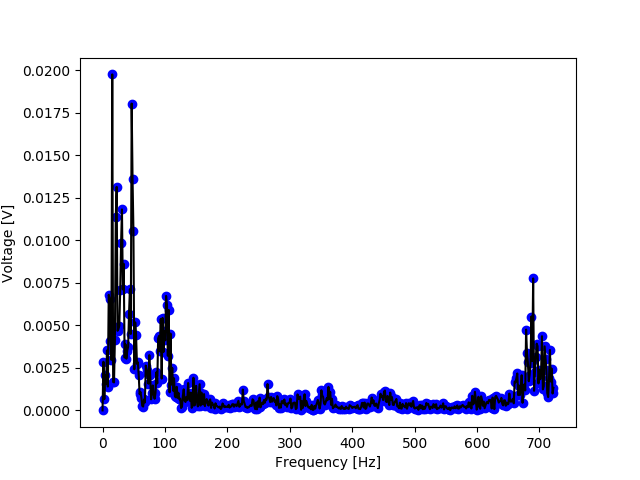
\includegraphics[width=\textwidth]{Experiment/Figs/3000_rpm_1khz_sterbina.png}
                \caption {Amplitudové spektrum ložiska s trhlinou.}
            \end{subfigure}
        \end{figure} 
        \begin{figure}[!ht]
            \centering
    	    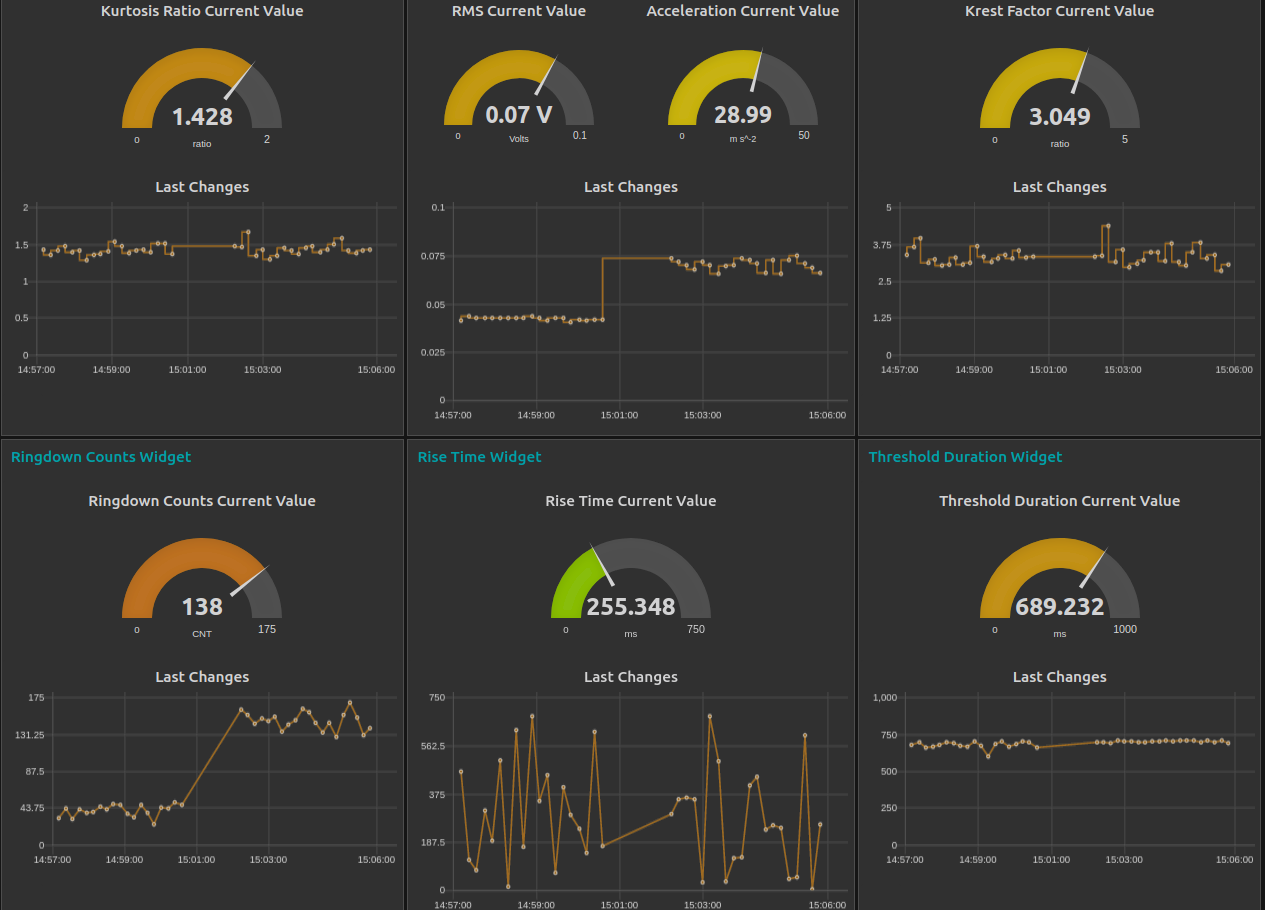
\includegraphics[width=\textwidth]{Experiment/Figs/sterbina_300rpm_1khZ2.png}
            \caption {Druhý experiment – časové průběhy.}
            \label{figure:experiment_graphs02}
        \end{figure}
        

    
    \subsection{Výsledky}  
        Nakonec i v druhém experimentu se hodnoty kurtosis ratio a krest faktoru po přesunu akcelerometru na druhé ložisko nezměnily, i když přítomnost trhliny by pomocí nich měla být detekovatelná. Po diskusi s vedoucím práce jsme došli k závěru, že pro větší vypovídající hodnotu těchto příznaků, bychom potřebovali druhé referenční zařízení zcela bez poruchy. Dále by bylo třeba navrhnout pásmovou propust, která by vyfiltrovala signál od frekvence motoru a jejích vyšších harmonických složek, které výrazně převládají ve výpočtu, a nedovolují tak menším změnám, aby se projevily. Návrh digitálních filtrů byl ovšem nad zbylé časové možnosti.\\
        Změny se vyskytly v hodnotách RMS a ringdown counts, které se po přesunu akcelerometru na druhé ložisko zvýšily, což mělo ovšem zřejmě důvod ve větší blízkosti k motoru, a tudíž větší amplitudě vibrací, a nikoliv v přítomnosti trhliny.
        
        Amplitudové spektrum přineslo podobné výsledky jako v prvním experimentu, a i zde se tedy ukázalo jako lepší ukazatel.
        
     
        
        